Создание SSH-ключа для возможности подключиться к удалённому репозиторию происходит в несколько этапов.
Для начала нужно проверить наличие ключа, введя следующие команды:
\newline \texttt{cd ~/.ssh}
\newline \texttt{ls}

Если файлов с названиями \texttt{id\_dsa} и \texttt{id\_dsa.pub} нет (открытый и приватный ключ), то можно создать их используя команду:
\newline  \texttt{ssh-keygen -o}
\newline \quad Далее нужно открыть содержимое файла dsa.pub командой:
\newline  \texttt{cat ~/.ssh/id\_dsa.pub}

Далее добавили свой ключ себе в аккаунт на GitHub, чтобы иметь возможность подключиться к удалённому репозиторию [2]. А также прописали ещё одну команду, необходимую для подключения.

\begin{figure}[h]
		\centering
		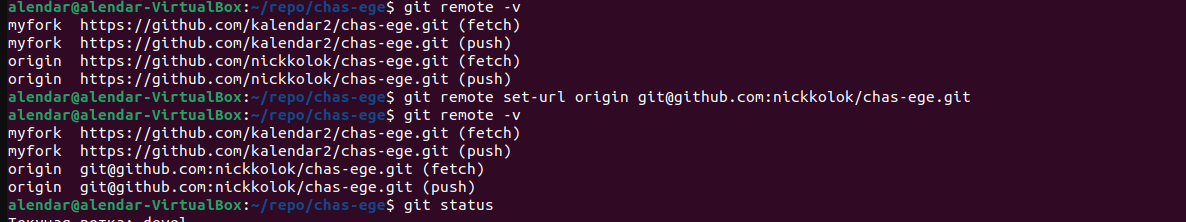
\includegraphics[width=1\linewidth]{VM/pod.png}
\caption{Подключению к удалённому репозиторию с помощью команды.}
\label{ris:image}
\end{figure}

Переходим в репозиторий на GitHub «ЧАС-ЕГЭ» и нажимаем кнопку «Fork» справа вверху.

Открыв VirtualBox и войдя в свою виртуальную машину, открыли терминал и перешли в папку с «Час ЕГЭ» с помошью команды cd git/chas-ege.

Представление гиту выглядит следующим образом:
\newline \texttt{git config ---global user.name «Фамилия Имя»}
\newline \texttt{git config ---global user.email «электронная почта пользователя»}
\newline Можно придать выводу гита красные и зелёные цвета с помощью команд:
\texttt{git config ---global color.ui true}
\newline Добавление своего форка на гитхаб в список удалённых репозиториев:
\texttt{git remote add myfork git@github.com:«GitHubNik»/chas-ege.git}, где «GitHubNik» - ник пользователя на гитхабе. 

Основные команды для создания и отправления изменений в удалённый репозиторий:
\\Переключение на основную ветку (devel):
\\ \texttt{git checkout devel}
\\ \quad Её обновление (В некоторых случаях применима также команда: \texttt{git pull origin devel}):
\\ \texttt{git fetch origin devel}
\\ \quad Создание новой ветки:
\\ \texttt{git checkout -b newtask-777}
\\ \quad Проверка изменений, а также самой ветки:
\\ \texttt{git status}
\\ \quad Добавление всех изменений:
\\ \texttt{git add .}
\\ \quad Добавление всех изменений:
\\ \texttt{git commit -m «Внесены изменения в файл ...»}
\\ \quad Отправка изменений в удалённый репозиторий:
\\ \texttt{git push myfork newtask-777:myfork newtask-777:}
